%%% Ne pas modifier jusqu'à la ligne 25
\documentclass[a4paper,12pt]{book}
\usepackage[utf8]{inputenc}
\usepackage[french]{babel}
%%\usepackage{CJK}
\usepackage{yhmath}
\usepackage[left=2cm,right=2cm,top=3cm,bottom=2cm, headheight=1.5cm,headsep=1.5cm]{geometry}
%%\usepackage{CJKutf8}
\usepackage{amsfonts}
\usepackage{mathrsfs}
\usepackage{amsmath,amsfonts,amssymb,dsfont}
\usepackage{graphicx}
\usepackage{subfigure}
\usepackage{enumitem}		%\enumerate-resume
\usepackage[colorlinks=true,unicode={true},hyperindex=false, linkcolor=blue, urlcolor=blue]{hyperref}
\newcommand{\myref}[1]{\ref{#1} page \pageref{#1}}

\addto\captionsfrench{\def\tablename{Tableau}}  %légendes des tableaux
\renewcommand\thesection{\Roman{section}~-~} 
\renewcommand\thesubsection{\Roman{section}.\Alph{subsection}~-~} 
\renewcommand\thesubsubsection{\Roman{section}.\Alph{subsection}.\arabic{subsubsection}~-~} 

\newcommand{\conclusion}[1]{\newline \centerline{\fbox{#1}}}

\setcounter{secnumdepth}{3}
\parindent=0pt

\usepackage{fancyhdr}
\pagestyle{fancy}

\lhead{SJTU-ParisTech} 
%%%%%%%%%%%%%%%%%%%%%%%%%%%%%%%%%%
\chead{TR15}
\rhead{Daniel 518261910024}

\begin{document}
\renewcommand{\labelitemi}{$\blacktriangleright$}
\renewcommand{\labelitemii}{$\bullet$}


\section{Principe de Huygens-Fresnel (formulation moderne)}
\begin{figure}[h]
    \begin{center}
    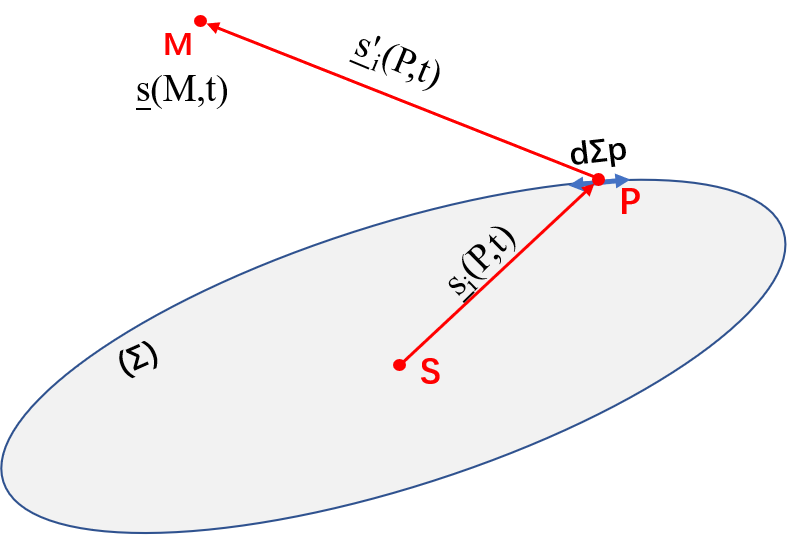
\includegraphics[scale=0.7]{tr151.png}
    \end{center}
    \caption{Figure du système}
\end{figure}
Pour une source ponctuelle monochromatique $S$ entourée d'une surface $(\Sigma)$. 
$(\Sigma)$ peut être décomposée en éléments de surface $d\Sigma_P$ centré autour de
points P. 

Le signal reçu en $P$ s'écrit $\underline{s}_i(P,t) = \underline{A}_i(P)e^{i\omega t}$, 
avec $\underline{A}_i(P)$ l'amplitude complexe, $\omega$ la pulsation de la source $S$

On peur considérer chaque élément de surface $d\Sigma_P$ comme une source secondaire ponctuelle qui émet
des ondes sphériques. Les ondes issues de $d\Sigma_P$ ont la même pulsation $\omega$ que la source, 
est elles ont un déphasage nul avec l'onde incidente en P.
Ses amplitudes sont proportionnelles à celle de l'onde incidente à la surface $d\Sigma_P$.

On obtient donc le signal émis par $d\Sigma_P$ est
$$
\underline{s}_i^{'}(P,t)=K\underline{A}_i(P)e^{i\omega t}\,d\Sigma_P
$$

Donc le signal $\underline{s}(M, t)$ reçu en un point M étudié est la superposition des signaux émis
par toutes les sources secondaires ponctuelles $P$, et les ondes sont incoincohérentes entre eux. 

En faisant la superposition, on obtiene le signal reçu par M
$$
\boxed{\underline{s}(M,t)=\iint_{(\Sigma)}K*\underline{A}_i(P)e^{i(\omega t-\varphi(M))}\,d\Sigma_P}
$$
avec $\varphi(M)=k_0(PM)=\frac{2\pi}{\lambda_0}(PM)$ le déphasage, K est une constante de proportionnalité homogène à l'inverse d'une surface, 
\subsection{L’amplitude diffractée}
\begin{figure}[h]
    \begin{center}
    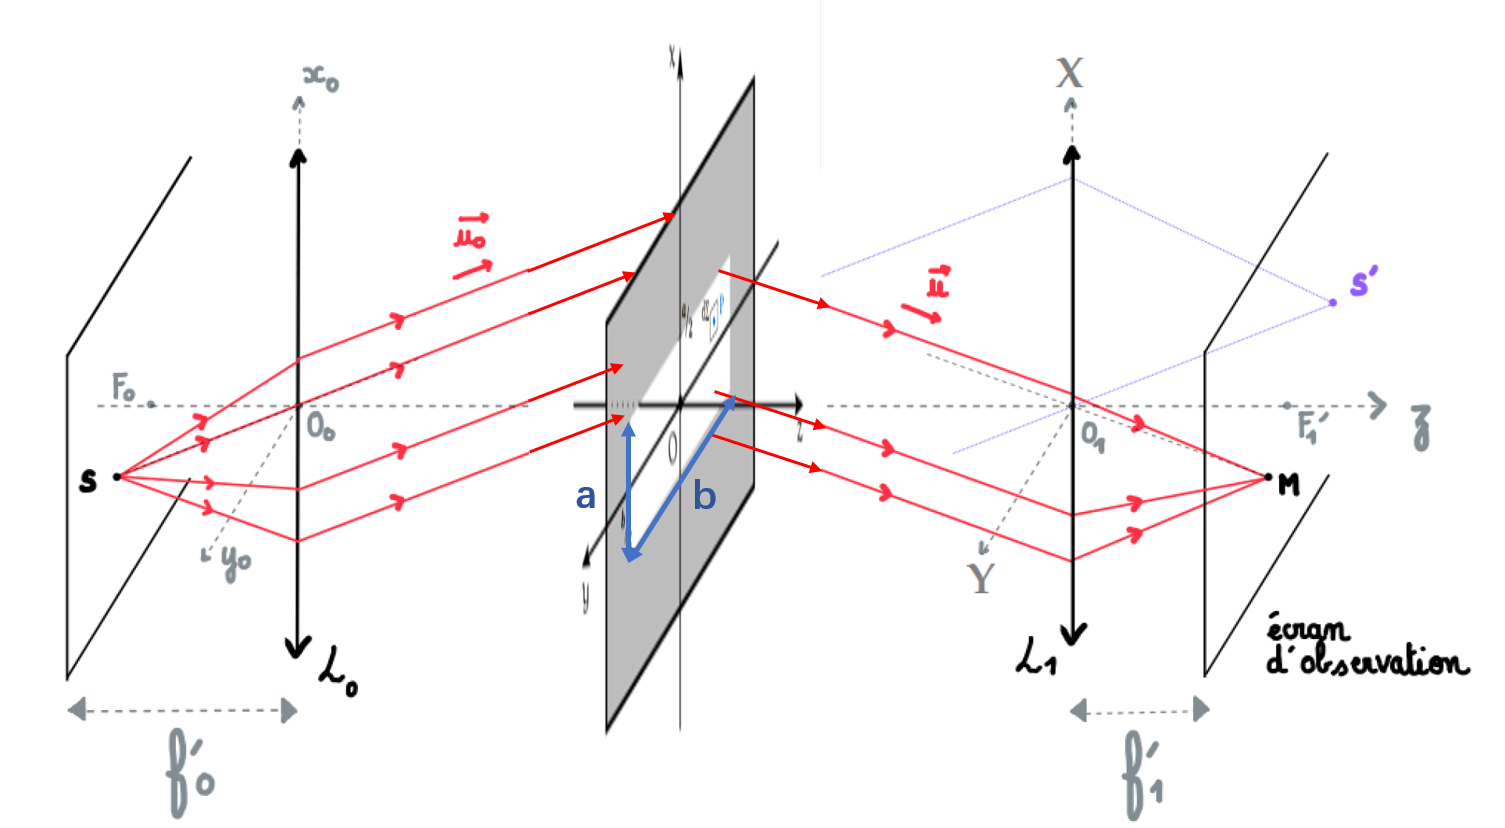
\includegraphics[scale=0.6]{tr152.png}
    \end{center}
    \caption{L’amplitude diffractée pour conditions de Fraunhofer}
\end{figure}
On a déjà en point M, l'amplitude complexe s'écrit
$$
\underline{A}_{diff}(M)=\underline{A}_{diff}(\alpha,\beta)=K\underline{A}_0\int^{x=\frac{a}{2}}_{x=-\frac{a}{2}}\int^{y=\frac{b}{2}}_{y=-\frac{b}{2}}e^{-\frac{2i\pi}{\lambda_0}[(\alpha_0-\alpha)x+(\beta_0-\beta)y]}\,dxdy
$$
Selon le théorème de Fubini, on a donc 
$$
\underline{A}_{diff}(M)=K\underline{A}_0\int^{x=\frac{a}{2}}_{x=-\frac{a}{2}}e^{-\frac{2i\pi}{\lambda_0}[(\alpha_0-\alpha)x]}\,dx\int^{y=\frac{b}{2}}_{y=-\frac{b}{2}}e^{-\frac{2i\pi}{\lambda_0}[(\beta_0-\beta)y]}\,dy
$$
On a donc 
\begin{align*}
\int^{x=\frac{a}{2}}_{x=-\frac{a}{2}}e^{-\frac{2i\pi}{\lambda_0}[(\alpha_0-\alpha)x]}\,dx&=\left[\frac{1}{-\frac{2i\pi}{\lambda_0}(\alpha_0-\alpha)}e^{-\frac{2i\pi}{\lambda_0}[(\alpha_0-\alpha)x]}\right]^{\frac{a}{2}}_{-\frac{a}{2}}\\
&=\frac{1}{-\frac{2i\pi}{\lambda_0}(\alpha_0-\alpha)}\left(e^{-\frac{i\pi}{\lambda_0}[(\alpha_0-\alpha)a]}-e^{\frac{i\pi}{\lambda_0}[(\alpha_0-\alpha)a]}\right)\\
&=\frac{1}{-\frac{2i\pi}{\lambda_0}(\alpha_0-\alpha)}\left(-2i\sin(\frac{\pi}{\lambda_0}[(\alpha_0-\alpha)a])\right)\\
&=a\frac{\sin(\frac{a\pi}{\lambda_0}(\alpha_0-\alpha))}{\frac{a\pi}{\lambda_0}(\alpha_0-\alpha)}\\
&=a\,sinc(\frac{a\pi}{\lambda_0}(\alpha_0-\alpha))
\end{align*}
De même,
$$
\int^{y=\frac{b}{2}}_{y=-\frac{b}{2}}e^{-\frac{2i\pi}{\lambda_0}[(\beta_0-\beta)y]}\,dy=b\,sinc(\frac{b\pi}{\lambda_0}(\beta_0-\beta))
$$
Donc 
$$
\boxed{\underline{A}_{diff}(M)=K\underline{A}_0ab\,sinc(\frac{a\pi}{\lambda_0}(\alpha_0-\alpha))\,sinc(\frac{b\pi}{\lambda_0}(\beta_0-\beta))}
$$
Donc dans le cas de la diffraction à l'infini d'une onde monochromatique plane par une ouverture rectangulaire de
surface $ab$, l'éclairement obtenu sur l'écran s'écrit
\begin{align*}
\mathcal{E}(M)&=\underline{A}_{diff}(M)\underline{A}^{*}_{diff}(M)\\
&=K^2\underline{A}_0\underline{A}_0^{*}a^2b^2\,sinc^2(\frac{a\pi}{\lambda_0}(\alpha_0-\alpha))\,sinc^2(\frac{b\pi}{\lambda_0}(\beta_0-\beta))\\
&=\boxed{\mathcal{E}_{max}\,sinc^2(\frac{a\pi}{\lambda_0}(\alpha_0-\alpha))\,sinc^2(\frac{b\pi}{\lambda_0}(\beta_0-\beta))}
\end{align*}
avec $\mathcal{E}_{max}=K^2|\underline{A}_0|^2a^2b^2$, l'éclairement maximal, obtenu dans la direction de l'optique géométrique$(\alpha=\alpha_0,\beta=\beta_0)$
\end{document}